\documentclass[final]{beamer}

% ====================
% Packages
% ====================

\usepackage[T1]{fontenc}
\usepackage{lmodern}
\usepackage[orientation=portrait,size=a0,scale=1.0]{beamerposter}
\usetheme{gemini}
\usecolortheme{nott}
\usepackage{graphicx}
\usepackage{booktabs}
\usepackage{tikz}
\usepackage{pgfplots}
\pgfplotsset{compat=1.14}
\usepackage{anyfontsize}
\usepackage{xcolor}
\usepackage[skip=2pt,font=normalsize]{subcaption}
\usepackage{adjustbox}

% ----------------------------------
% For plotting study methodology
% ----------------------------------

\usepackage{tikz}
\usetikzlibrary{shapes.geometric, arrows}

% Defining Tickz Style
\tikzstyle{startstop} = [rectangle, rounded corners, minimum width=3cm, minimum height=1cm, text centered, text width = 10cm, draw=black, fill=white]

% \tikzstyle{io} = [trapezium, trapezium left angle=70, trapezium right angle=110, minimum width=3cm, minimum height=1cm, text centered, text width = 4.5cm, draw=black, fill=blue!30]

\tikzstyle{process} = [rectangle, minimum width=3cm, minimum height=1cm, text centered, text width = 6cm, draw=black, fill=white, text width = 10cm]

% \tikzstyle{decision} = [diamond, minimum width=3cm, minimum height=1cm, text centered, draw=black, fill=green!30]

\tikzstyle{arrow} = [ultra thick,->,>=stealth]


% ====================
% Lengths
% ====================

% If you have N columns, choose \sepwidth and \colwidth such that
% (N+1)*\sepwidth + N*\colwidth = \paperwidth
\newlength{\sepwidth}
\newlength{\colwidth}
\setlength{\sepwidth}{0.025\paperwidth}
\setlength{\colwidth}{0.45\paperwidth}

\newcommand{\separatorcolumn}{\begin{column}{\sepwidth}\end{column}}

% ====================
% Title
% ====================

\title{Exploring new tendencies in numerical optimization applied to PINNs. An example with the nonlinear time-dependent Schrödinger's Equation.}

\author{Cruz, Díaz Emmanuel \inst{1} \and Velazquez, Castro Jorge \inst{2}}

\institute[shortinst]{\inst{1,}\inst{2} Facultad de Ciencias Físico Matemáticas, Benemérita Universidad Autónoma de Puebla \samelineand}

% ====================
% Footer (optional)
% ====================

%\footercontent{
  %\href{https://www.lipsum.com}{\textbf{https://www.lipsum.com}} \hfill
  %\textbf{Ph.D. Connect Conclave 2023} \hfill
  %\href{mailto:your.email@provider.com}{\textbf{your.email@provider.com}}}
% (can be left out to remove footer)


% ====================
% Logo (optional)
% ====================

% use this to include logos on the left and/or right side of the header:
\logoright{
\includegraphics[height=6.3cm]{fcfm-w.png}}
\logoleft{
\includegraphics[height=7cm]{BUAP-w.png}}

% ====================
% Body
% ====================

\begin{document}

\begin{frame}[t]
\begin{columns}[t]
\separatorcolumn

\begin{column}{\colwidth}

% ----------------------------------
% Abstract
% ----------------------------------
  \begin{block}{Abstract}
    Recientemente las \textit{Physics Informed Neural Networks (PINN)} han surgido como una alternativa muy poderosa
    para la resolución de problemas numéricos directos e inversos. Empero, el estado del arte del diseño de las PINNs se ha visto
    estancado en el uso de optimizadores como Adam o SGD junto con optimizadores quasi-Newtonianos como el LBFGS. Este trabajo
    explora las nuevas tendencias en optimización numérica, típicamente empleadas en modelos largos de lenguaje (LLM) y una 
    propuesta de optimizador LBFGSAdam que aprovecha lo mejor de ambos optimizadores. El problema atacado para explorar estas nuevas
    tendencias en optimización es la ecuación de Schrödinger no lineal dependiente del tiempo. Los resultados muestran que estas nuevas
    alternativas para optimizar la función de costo de las PINNs son favorables y que estos optimizadores permiten obtener una mayor precisión
    que el estado de arte actual de las PINNs, muy a pesar de que su diseño no haya sido precisamente enfocado para este propósito.     
  \end{block}
  
% ----------------------------------
% Sección: PINNs
% ----------------------------------
  \begin{block}{Physics Informed Neural Networks}

    Las redes neuronales informadas de la física (PINN) fueron introducidas por primera vez por M. Raissi et al. en \cite{Raissi2019}. 
    Resultaron como una propuesta para 

    \heading{Research gaps}
    si
  \end{block}



% -------------------------------
% Section: Conclusiones
% -------------------------------
   \begin{block}{Conclusiones}
    sí
  \end{block}

% -------------------------------
% Section: Referencias
% ------------------------------- 

  \begin{block}{Referencias}

    \nocite{*}
    \footnotesize{\bibliographystyle{plain}\bibliography{poster}}

  \end{block}

% -------------------------------
% Section: Portfolio
% -------------------------------
  \begin{block}{Author$^{1}$ Portfolio Website}
    
    \begin{figure}[h]
    \centering
    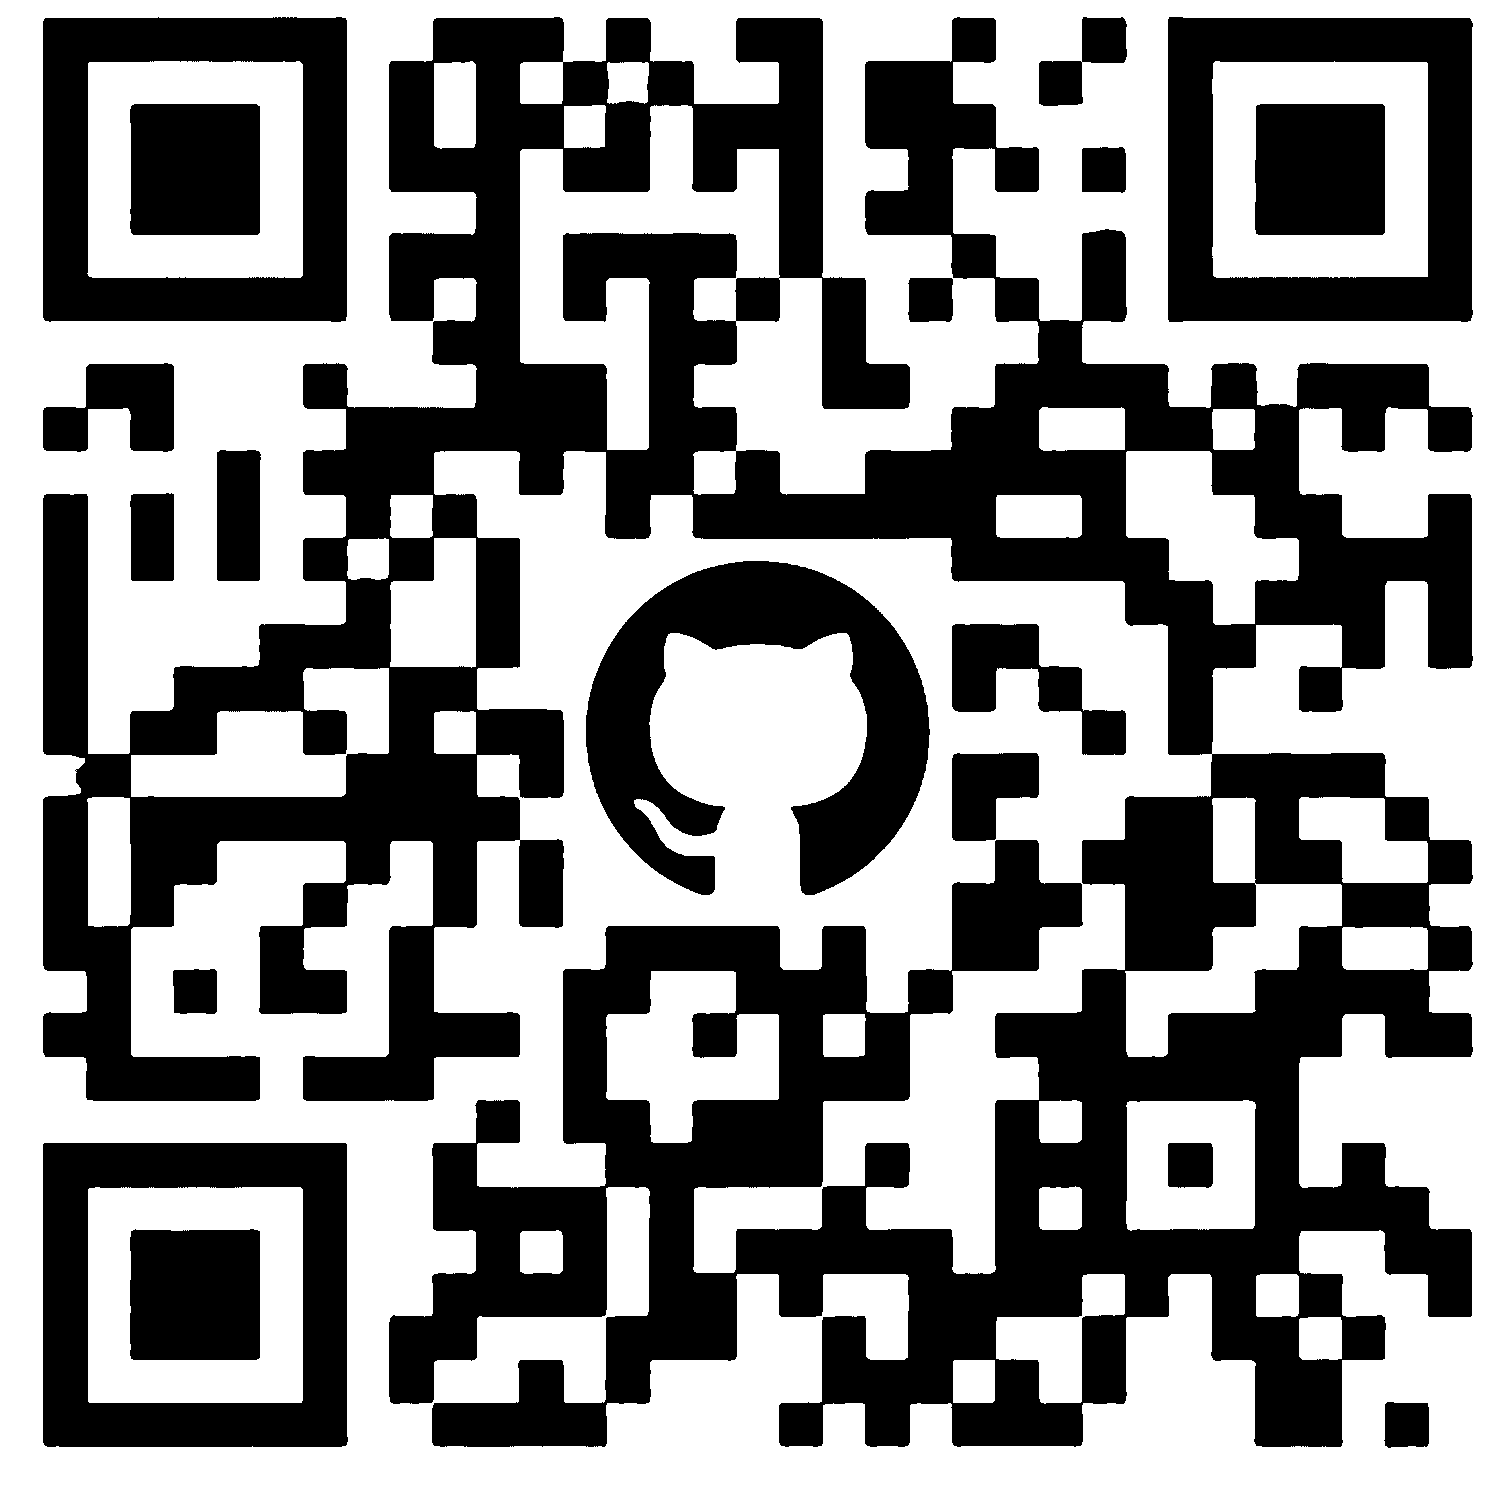
\includegraphics[width=0.1\textwidth]{images/QR.png}
    \caption*{Scan this QR code}
    \label{fig:figure3}
\end{figure}

  \end{block}

\end{column}
\separatorcolumn



\end{columns}
\end{frame}

\end{document}
